%%%%%%%%%%%%%%%%%%%%%%%%%%%%%%%%%%%%%%%%%%%%%%%%%%%%%%%%%%%%%%%
%
% Welcome to writeLaTeX --- just edit your LaTeX on the left,
% and we'll compile it for you on the right. If you give
% someone the link to this page, they can edit at the same
% time. See the help menu above for more info. Enjoy!
%
%%%%%%%%%%%%%%%%%%%%%%%%%%%%%%%%%%%%%%%%%%%%%%%%%%%%%%%%%%%%%%%

% --------------------------------------------------------------
% This is all preamble stuff that you don't have to worry about.
% Head down to where it says "Start here"
% --------------------------------------------------------------
 
\documentclass[12pt]{article}
 
\usepackage[margin=1in]{geometry}
\usepackage{amsmath,amsthm,amssymb}

\usepackage{listings}
\usepackage{xcolor}
\usepackage{circuitikz}
\usetikzlibrary{bending}
\usetikzlibrary{patterns,decorations.pathmorphing,positioning}
\usepackage{float,graphicx}

%New colors defined below
\definecolor{codegreen}{rgb}{0,0.6,0}
\definecolor{codegray}{rgb}{0.5,0.5,0.5}
\definecolor{codepurple}{rgb}{0.58,0,0.82}
\definecolor{backcolour}{rgb}{0.95,0.95,0.92}

%Code listing style named "mystyle"
\lstdefinestyle{mystyle}{
  backgroundcolor=\color{backcolour}, commentstyle=\color{codegreen},
  keywordstyle=\color{magenta},
  numberstyle=\tiny\color{codegray},
  stringstyle=\color{codepurple},
  basicstyle=\ttfamily\footnotesize,
  breakatwhitespace=false,         
  breaklines=true,                 
  captionpos=b,                    
  keepspaces=true,                 
  numbers=left,                    
  numbersep=5pt,                  
  showspaces=false,                
  showstringspaces=false,
  showtabs=false,                  
  tabsize=2
}

%"mystyle" code listing set
\lstset{style=mystyle}

 
\newcommand{\N}{\mathbb{N}}
\newcommand{\Z}{\mathbb{Z}}
 
\newenvironment{theorem}[2][Theorem]{\begin{trivlist}
\item[\hskip \labelsep {\bfseries #1}\hskip \labelsep {\bfseries #2.}]}{\end{trivlist}}
\newenvironment{lemma}[2][Lemma]{\begin{trivlist}
\item[\hskip \labelsep {\bfseries #1}\hskip \labelsep {\bfseries #2.}]}{\end{trivlist}}
\newenvironment{exercise}[2][Exercise]{\begin{trivlist}
\item[\hskip \labelsep {\bfseries #1}\hskip \labelsep {\bfseries #2.}]}{\end{trivlist}}
\newenvironment{problem}[2][Problem]{\begin{trivlist}
\item[\hskip \labelsep {\bfseries #1}\hskip \labelsep {\bfseries #2.}]}{\end{trivlist}}
\newenvironment{question}[2][Question]{\begin{trivlist}
\item[\hskip \labelsep {\bfseries #1}\hskip \labelsep {\bfseries #2.}]}{\end{trivlist}}
\newenvironment{corollary}[2][Corollary]{\begin{trivlist}
\item[\hskip \labelsep {\bfseries #1}\hskip \labelsep {\bfseries #2.}]}{\end{trivlist}}

\newenvironment{solution}{\begin{proof}[Solution]}{\end{proof}}
 
\begin{document}
 
% --------------------------------------------------------------
%                         Start here
% --------------------------------------------------------------
 
\title{Lab 1}%replace X with the appropriate number
\author{Mengxiang Jiang\\ %replace with your name
CSEN 5303 Cybersecurity} %if necessary, replace with your course title
 
\maketitle
 
\begin{problem}{1} %You can use theorem, exercise, problem, or question here.  Modify x.yz to be whatever number you are proving
Free Antimalware

\begin{enumerate}
    \item Launch a web browser and navigate to the Malwarebytes website (\textbf{www.malewarebytes.com}). Locate and download the free home home version of the software, and install it on your virtual machine.
    \begin{figure}[H]
        \centering
        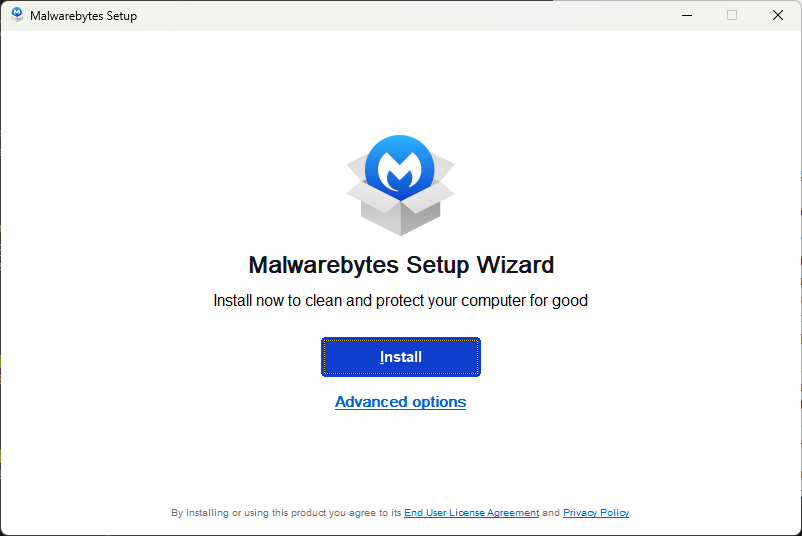
\includegraphics[width=0.8\textwidth]{install1}
        \caption{Malwarebytes Installer Start Screen}
    \end{figure}
    \begin{figure}[H]
        \centering
        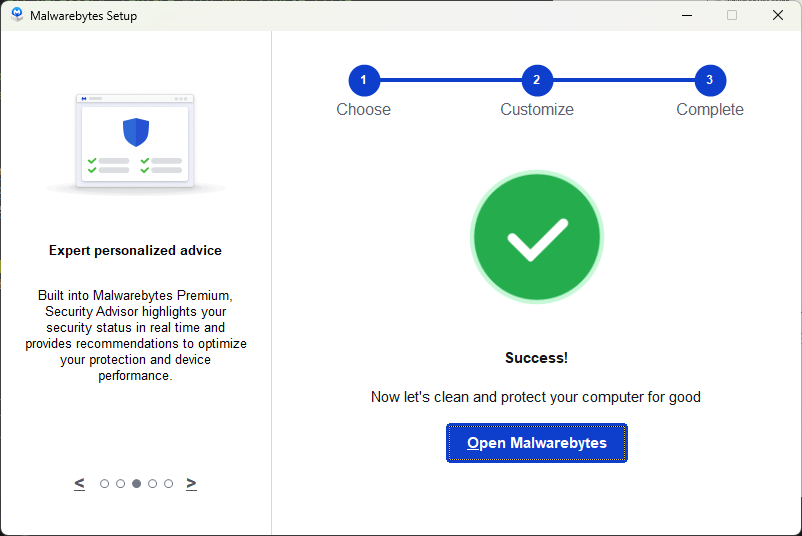
\includegraphics[width=0.8\textwidth]{install2}
        \caption{Malwarebytes Installer Completion Screen}
    \end{figure}
    \item Launch Malwarebytes and check for updates. If not current, get the latest virus definitions.
    \begin{figure}[H]
        \centering
        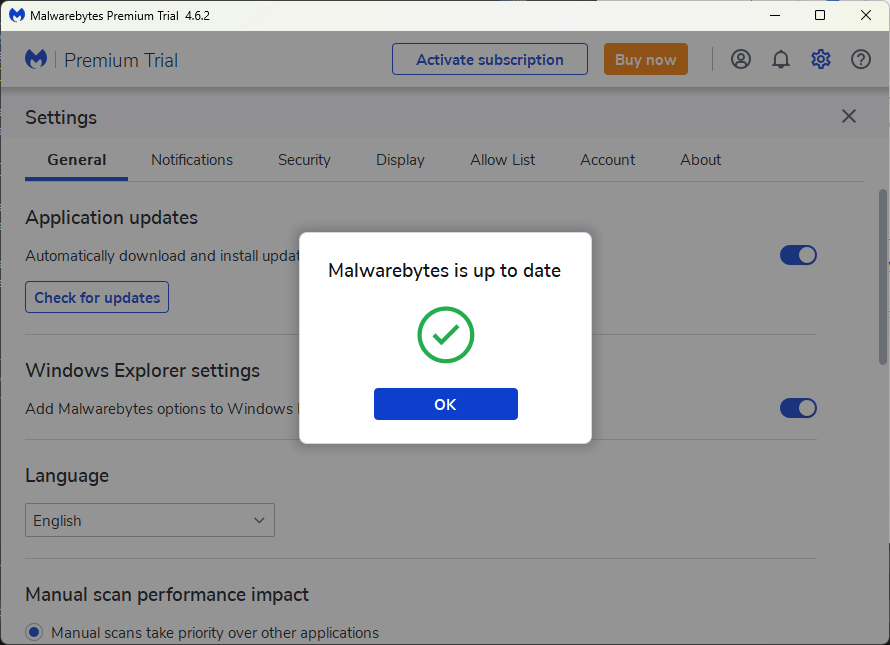
\includegraphics[width=0.8\textwidth]{update}
        \caption{Malwarebytes Update Screen}
    \end{figure}
    \item Scan your computer with Malewarebytes. Wait for the scan to complete.
    \begin{figure}[H]
        \centering
        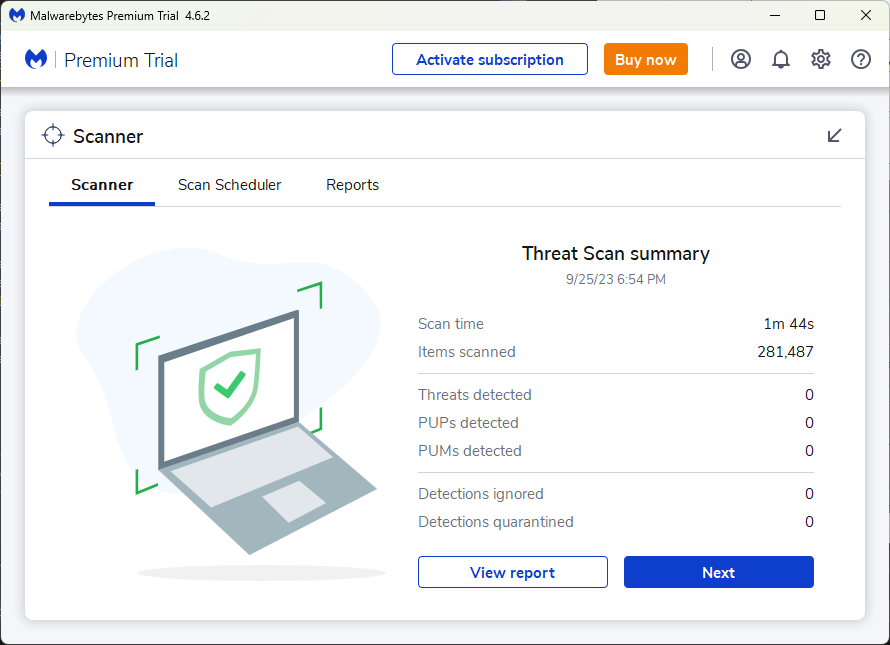
\includegraphics[width=0.8\textwidth]{scan}
        \caption{Malwarebytes Scan Complete Screen}
    \end{figure}
    \pagebreak
    \item Create and save a screenshot of the results. How many threats were identified on your machine?
    \begin{figure}[H]
        \centering
        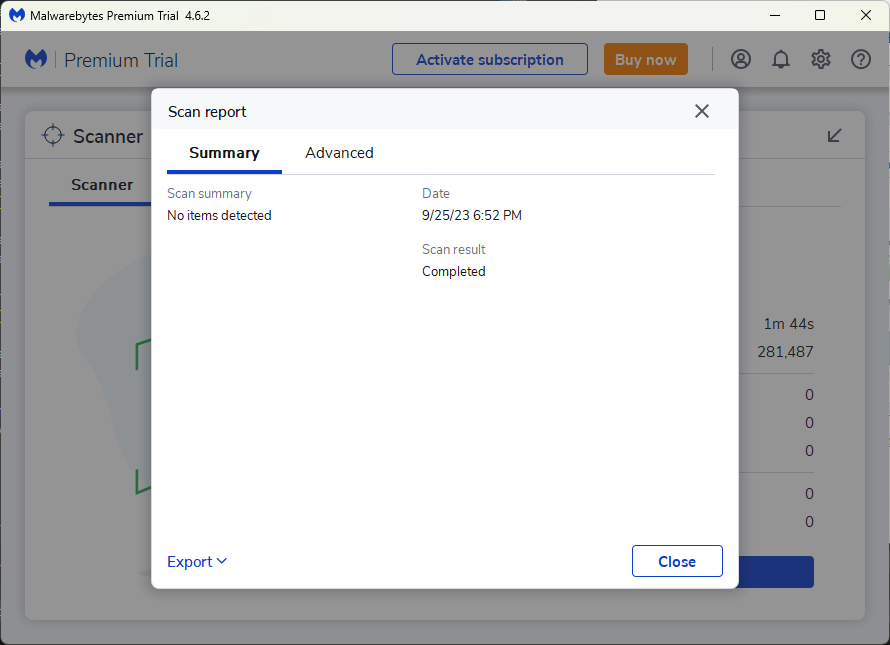
\includegraphics[width=0.8\textwidth]{report}
        \caption{Malwarebytes Scan Report}
    \end{figure}
    No threats were identified.
    \item Review any potentially malicious files that were identified, and quarantine those you believe are malicious. If you are not sure, the safest option is to quarantine the file.\\\\
    Since no threats were identified, I did nothing for this step.
    \pagebreak
    \item Locate the setting options for Malwarebytes. Does Malwarebytes scan for rootkits by default?
    \begin{figure}[H]
        \centering
        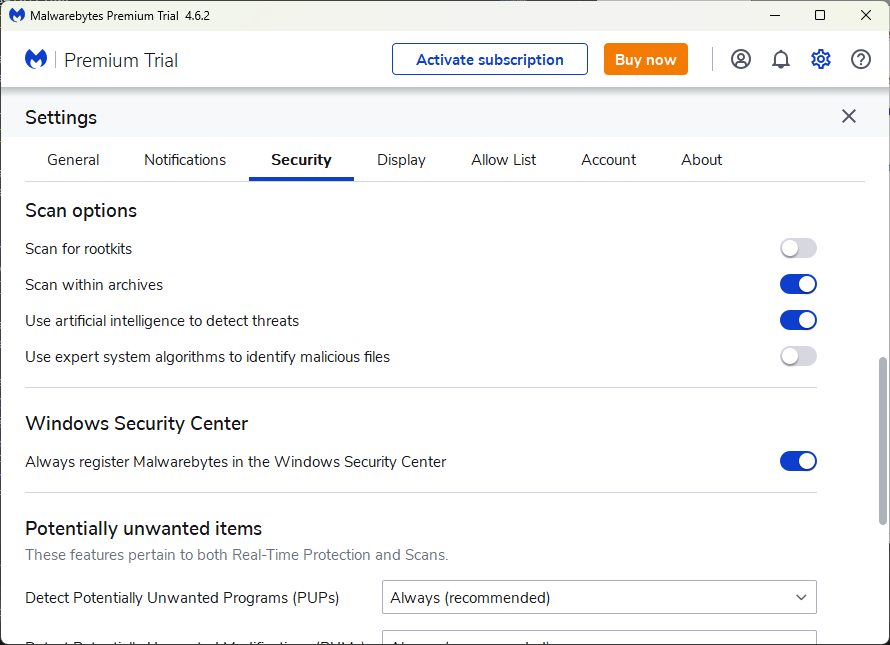
\includegraphics[width=0.8\textwidth]{rootkit}
        \caption{Malwarebytes Scan Options}
    \end{figure}
    Rootkits are not scanned by default.
    \pagebreak
    \item What does PUP stand for?
    \begin{figure}[H]
        \centering
        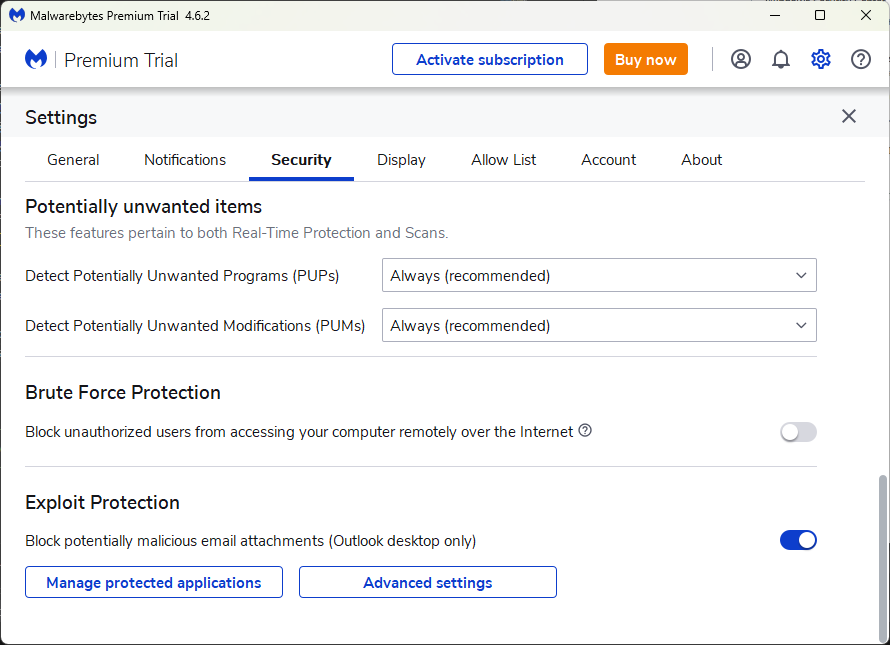
\includegraphics[width=0.8\textwidth]{pup}
        \caption{Malwarebytes PUP}
    \end{figure}
    PUP stands for Potentially Unwanted Programs
    \pagebreak
    \item What is the default schedule for Malwarebytes to perform a scan?
    \begin{figure}[H]
        \centering
        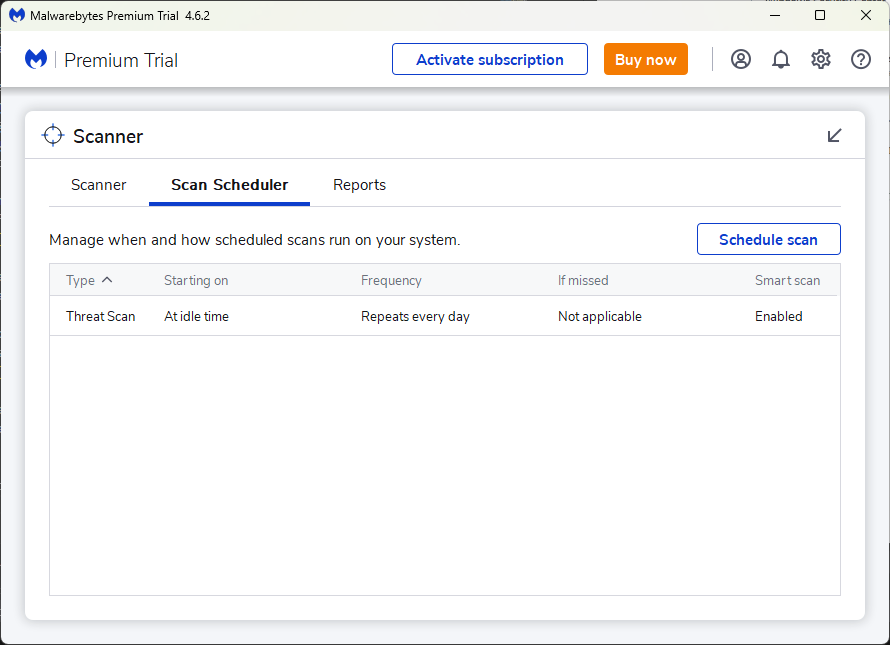
\includegraphics[width=0.8\textwidth]{schedule}
        \caption{Malwarebytes Scan Scheduler}
    \end{figure}
    The default schedule says at idle time everyday.
\end{enumerate}

\end{problem}
% --------------------------------------------------------------
%     You don't have to mess with anything below this line.
% --------------------------------------------------------------
 
\end{document}